\begin{exercise}{Le slinky au repos}{2}{Sup}
{Mécanique,Oscillateur harmonique,Ressort}{lelay}

À la fin de cet exercice, on aura modélisé la forme au repos d'un slinky (les grands ressorts qui descendent les escaliers tous seuls).
\begin{questions}
    \questioncours Force exercée par un ressort. Lois d'association de ressorts.
    \uplevel{On considère un assemblage constitué d'un mobile de masse $m_1$, reliée horizontalement à un mur situé en $x = 0$ par un ressort de raideur $k_1$ et de longueur à vide $\ell_1$. On repère la position de la masse par rapport au mur et on l'appelle $x(t)$.}
    \begin{center}
    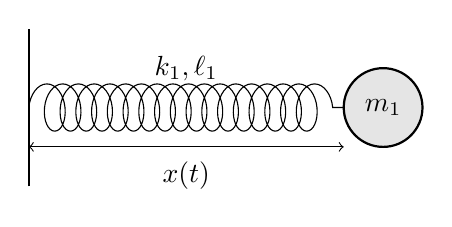
\begin{tikzpicture}
    
    \draw[thick, black] (0,-1) -- (0,1);
    
    \draw[decoration={aspect=0.6, segment length=2mm, amplitude=3mm,coil},decorate] (0,0) -- (4,0);
    \draw (2,0) node[above=6pt] {$k_1, \ell_1$};
    
    \filldraw[thick, color=black, fill=black!10] (4.5,0) circle (0.5);
    \draw (4.5,0) node {$m_1$};
    
    \draw[<->] (0,-0.5) -- (4,-0.5);
    \draw (2,-0.5) node[below=2pt] {$x(t)$};
    
    \end{tikzpicture}
    \end{center}
    \question Décrire qualitativement puis quantitativement les mouvements de perturbation d'amplitude initiale $y_0$ autour de la position de repos de la masse ? On appellera $y$ l'écart à l'équilibre.
    \question Comment évolue ce résultat si on suppose que le ressort est maintenant vertical et soumis à la gravité $g$ ?
    \uplevel{Cette fois-ci on utilise deux mobiles de masse $m_2$ et deux ressorts, de raideur $k_2$ et de longueur à vide $\ell_2$, comme dans l'illustration ci-dessous.}
    \begin{center}
    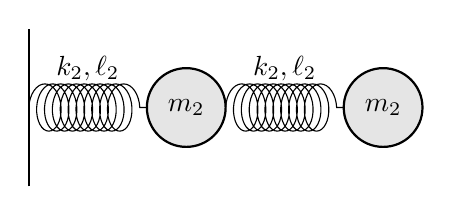
\begin{tikzpicture}
    
    \draw[thick, black] (0,-1) -- (0,1);
    
    \draw[decoration={aspect=0.6, segment length=1mm, amplitude=3mm,coil},decorate] (0,0) -- (1.5,0);
    \draw (0.75,0) node[above=6pt] {$k_2, \ell_2$};
    
    \filldraw[thick, color=black, fill=black!10] (2,0) circle (0.5);
    \draw (2,0) node {$m_2$};
    
    \draw[decoration={aspect=0.6, segment length=1mm, amplitude=3mm,coil},decorate] (2.5,0) -- (4,0);
    \draw (3.25,0) node[above=6pt] {$k_2, \ell_2$};
    
    
    \filldraw[thick, color=black, fill=black!10] (4.5,0) circle (0.5);
    \draw (4.5,0) node {$m_2$};
    
    \end{tikzpicture}
    \end{center}
    \question Que doivent valoir $m_2$ et $\ell_2$ pour que la position au repos de la masse la plus à droite et la masse totale soient les mêmes que précédemment ?
    \question On maintient la masse la plus à droite à une distance $y$ de sa position d'équilibre.
    \begin{parts}
        \part À l'équilibre, quelle est la position de la masse du milieu ? 
        \part Quelle est la force exercée par le ressort le plus à droite sur la masse la plus à droite ?
        \part Que doit valoir $k_2$ pour que cette force soit la même qu'avec l'assemblage précédent ?
    \end{parts}
    \question Comment choisir $\ell_n$, $m_n$ et $k_n$ dans le cas de $n$ masses ?
    
    \uplevel{On considère maintenant le même assemblage de deux masses $m_2$ que précédemment, mais cette fois à la verticale.}
    \question Quelle est la position d'équilibre de chaque ressort ?
    \question S'il y en a maintenant $n$, comment évolue l'écart entre chaque spire ?
\end{questions}
\end{exercise}
